%----------------------------------------------------------------------------------------
%	PACKAGES AND THEMES
%----------------------------------------------------------------------------------------
\pdfoutput=1
\documentclass[swedish]{beamer}

\usepackage[utf8]{inputenc}
\usepackage[scaled]{helvet} %helvetica i sliden blir bra
\usepackage[T1]{fontenc}

\usepackage{graphicx} % Allows including images
\usepackage{booktabs} % Allows the use of \toprule, \midrule and \bottomrule in tables
\usepackage{comment}
\usepackage[swedish]{babel}
\usepackage{graphicx}
\usepackage{graphics}
\usepackage{units}
%\usepackage{siunitx} %SI-enheter
\usepackage{comment}
\usepackage{epstopdf}
\usepackage{tikz}
\usepackage{eso-pic}
\usepackage{wallpaper} %För bakgrundsbilder
\usepackage{multimedia}
\usepackage{media9}

\usepackage{physics}


\graphicspath{ 
{src_figures/Avancez/}  %specialbilder som bara behövs för bakgrunden
{figures/} %bilder som används i själva presentationen
}

\newcommand\impl{\stackrel{\mathclap{\normalfont\mbox{?}}}{\Longleftrightarrow}}



\definecolor{CTHblue}{RGB}{00,00,102}   % Dessa är faktiskt officella Chalmersfärger som är beslutat att
\definecolor{CTHgrey}{RGB}{204,204,204} % de skall användas till presentationer. Andra är inte tillåtna...
\definecolor{CTHgreen}{RGB}{113,178,60} % citation needed []
\definecolor{CTHblack}{RGB}{00,00,00}


\mode<presentation> {

% The Beamer class comes with a number of default slide themes
% which change the colors and layouts of slides. Below this is a list
% of all the themes, uncomment each in turn to see what they look like.

%\usetheme{default}
%\usetheme{AnnArbor}
%\usetheme{Antibes}
%\usetheme{Bergen}
%\usetheme{Berkeley}
%\usetheme{Berlin}
%\usetheme{Boadilla}
%\usetheme{CambridgeUS}
%\usetheme{Copenhagen}
%\usetheme{Darmstadt}
%\usetheme{Dresden}
%\usetheme{Frankfurt}
%\usetheme{Goettingen}
%\usetheme{Hannover}
%\usetheme{Ilmenau}
%\usetheme{JuanLesPins}
%\usetheme{Luebeck}
%\usetheme{Madrid}
%\usetheme{Malmoe}
%\usetheme{Marburg}
%\usetheme{Montpellier}
%\usetheme{PaloAlto}
%\usetheme{Pittsburgh}
%\usetheme{Rochester}
%\usetheme{Singapore}
%\usetheme{Szeged}
%\usetheme{Warsaw}

% As well as themes, the Beamer class has a number of color themes
% for any slide theme. Uncomment each of these in turn to see how it
% changes the colors of your current slide theme.

%\usecolortheme{albatross}
%\usecolortheme{beaver}
%\usecolortheme{beetle}
%\usecolortheme{crane}
%\usecolortheme{dolphin}
%\usecolortheme{dove}
%\usecolortheme{fly}
%\usecolortheme{lily}
%\usecolortheme{orchid}
%\usecolortheme{rose}
%\usecolortheme{seagull}
%\usecolortheme{seahorse}
%\usecolortheme{whale}
%\usecolortheme{wolverine}

% \setbeamercolor*{palette primary}{fg=CTHgrey,bg=CTHblue}
% \setbeamercolor*{palette secondary}{fg=CTHblack,bg=CTHgrey}
% \setbeamercolor*{palette tertiary}{fg=CTHgrey,bg=CTHblack}

%\setbeamertemplate{footline} % To remove the footer line in all slides uncomment this line
%\setbeamertemplate{footline}[page number] % To replace the footer line in all slides with a simple slide count uncomment this line

%\setbeamertemplate{navigation symbols}{} % To remove the navigation symbols from the bottom of all slides uncomment this line
}

\usepackage{custom_as}

\newcommand{\RBox}[1]{%
  \tikz\node[draw,rounded corners,align=center,] {#1};%
}  

% \usebackgroundtemplate{\vbox to \paperheight{\vspace*{2pt}\includegraphics[width=\paperwidth]{cth_fp.pdf}}}



\renewcommand{\thefootnote}{\fnsymbol{footnote}}

%----------------------------------------------------------------------------------------
%	TITLE PAGE
%----------------------------------------------------------------------------------------


\usetheme[titleflower=true]{chalmers} % titleflower = true or false
\title[Brownsk rörelse i celler]{Brownsk rörelse i celler hos partiklar och strängar} % Första klammern är en "short title"
\subtitle{} % optional
\author{Andréas Sundström \and Emelie Ekenstedt \and Robin Karlsson \and Oliver Sundell} % [short author (optional)]{many authors}
\institute[Chalmers]{Chalmers tekniska högskola, \\Institutionen för fysik, \\Avdelningen för biofysik}
%\titlepageextra{IPT 2015, Warsaw} % Optional extra info, appears before date on title page
\footer{\insertshorttitle} % optional, manually sets footer (default is short author)
%\footer{Something completely different} % but it can of course be anything.

\titlepagelogofile{Avancez_black}
\date{\vspace{-0.25cm}}

\usepackage{multimedia}


\begin{document}

\begin{frame}[plain]

\linethickness{0.075mm}

  \titlepage
\end{frame}
% }







%%%%%%%%%%%%%%%%%%%%%%%%Här börjar presentationen%%%%%%%%%%%%%%%%%%%%%%%%


\begin{frame}
\frametitle{Innehåll}

\tableofcontents

\end{frame}



\section{Cellbiologi}%detta kommer med i innehållsförteckningen 
\begin{frame}
\frametitle{Cellbiologi}
 \begin{columns}[c]
\column{.4\textwidth} % Left column and width


Cytoplasman
\vspace{8mm}

Aktinfilament
\vspace{8mm}

Diffusion, passiv transport

\column{.6\textwidth} % Right column and width

\begin{figure} %Filament kring kärnan
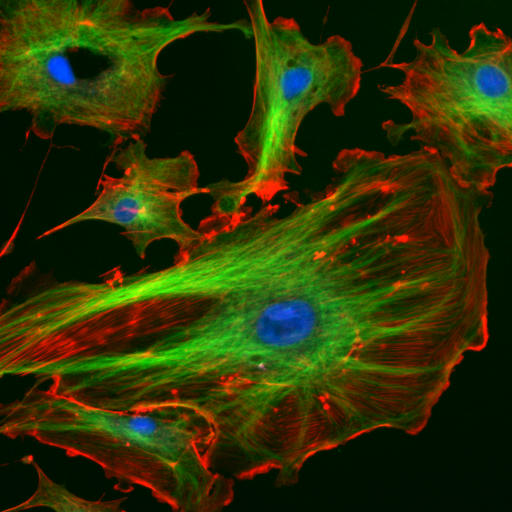
\includegraphics[width=1\textwidth]{figures/FluorescentCells.png}
\end{figure}
%https://commons.wikimedia.org/wiki/File:FluorescentCells.jpg

\end{columns}
\end{frame}



%%%%%%%%%%%%%%%
\section{Partikelrörelse}

\begin{frame}
\frametitle{Film av partiklar i jästceller}

\centering
\movie[width=7.35cm, height=4.08cm, poster=last]{}{filmer/partiklar_ed.avi}

\end{frame}


\begin{frame}
\frametitle{Partikelmodeller och MSD}
\begin{columns}[c]
\column{.5\textwidth} % Left column and width

Partikelmodeller:
\begin{itemize}[label={$\bullet$}]
    \item Brownsk rörelse
    \item CTRW -- continuous time random walk
    \item fBm -- fractional Brownian motion
\end{itemize}
%\\[1cm]
MSD:
%\vspace{-5mm}
\[
\ev{( x(t+\Delta{t})-x(t) )^2}
\]%\vspace{-5mm}
\[
\ev{( x(t)-x(0) )^2}
\]

\column{.5\textwidth} % Right column and width

\begin{figure} %MSD för dvala
\resizebox{1\textwidth}{!}{
% GNUPLOT: LaTeX picture with Postscript
\begingroup
  \makeatletter
  \providecommand\color[2][]{%
    \GenericError{(gnuplot) \space\space\space\@spaces}{%
      Package color not loaded in conjunction with
      terminal option `colourtext'%
    }{See the gnuplot documentation for explanation.%
    }{Either use 'blacktext' in gnuplot or load the package
      color.sty in LaTeX.}%
    \renewcommand\color[2][]{}%
  }%
  \providecommand\includegraphics[2][]{%
    \GenericError{(gnuplot) \space\space\space\@spaces}{%
      Package graphicx or graphics not loaded%
    }{See the gnuplot documentation for explanation.%
    }{The gnuplot epslatex terminal needs graphicx.sty or graphics.sty.}%
    \renewcommand\includegraphics[2][]{}%
  }%
  \providecommand\rotatebox[2]{#2}%
  \@ifundefined{ifGPcolor}{%
    \newif\ifGPcolor
    \GPcolortrue
  }{}%
  \@ifundefined{ifGPblacktext}{%
    \newif\ifGPblacktext
    \GPblacktexttrue
  }{}%
  % define a \g@addto@macro without @ in the name:
  \let\gplgaddtomacro\g@addto@macro
  % define empty templates for all commands taking text:
  \gdef\gplbacktext{}%
  \gdef\gplfronttext{}%
  \makeatother
  \ifGPblacktext
    % no textcolor at all
    \def\colorrgb#1{}%
    \def\colorgray#1{}%
  \else
    % gray or color?
    \ifGPcolor
      \def\colorrgb#1{\color[rgb]{#1}}%
      \def\colorgray#1{\color[gray]{#1}}%
      \expandafter\def\csname LTw\endcsname{\color{white}}%
      \expandafter\def\csname LTb\endcsname{\color{black}}%
      \expandafter\def\csname LTa\endcsname{\color{black}}%
      \expandafter\def\csname LT0\endcsname{\color[rgb]{1,0,0}}%
      \expandafter\def\csname LT1\endcsname{\color[rgb]{0,1,0}}%
      \expandafter\def\csname LT2\endcsname{\color[rgb]{0,0,1}}%
      \expandafter\def\csname LT3\endcsname{\color[rgb]{1,0,1}}%
      \expandafter\def\csname LT4\endcsname{\color[rgb]{0,1,1}}%
      \expandafter\def\csname LT5\endcsname{\color[rgb]{1,1,0}}%
      \expandafter\def\csname LT6\endcsname{\color[rgb]{0,0,0}}%
      \expandafter\def\csname LT7\endcsname{\color[rgb]{1,0.3,0}}%
      \expandafter\def\csname LT8\endcsname{\color[rgb]{0.5,0.5,0.5}}%
    \else
      % gray
      \def\colorrgb#1{\color{black}}%
      \def\colorgray#1{\color[gray]{#1}}%
      \expandafter\def\csname LTw\endcsname{\color{white}}%
      \expandafter\def\csname LTb\endcsname{\color{black}}%
      \expandafter\def\csname LTa\endcsname{\color{black}}%
      \expandafter\def\csname LT0\endcsname{\color{black}}%
      \expandafter\def\csname LT1\endcsname{\color{black}}%
      \expandafter\def\csname LT2\endcsname{\color{black}}%
      \expandafter\def\csname LT3\endcsname{\color{black}}%
      \expandafter\def\csname LT4\endcsname{\color{black}}%
      \expandafter\def\csname LT5\endcsname{\color{black}}%
      \expandafter\def\csname LT6\endcsname{\color{black}}%
      \expandafter\def\csname LT7\endcsname{\color{black}}%
      \expandafter\def\csname LT8\endcsname{\color{black}}%
    \fi
  \fi
  \setlength{\unitlength}{0.0500bp}%
  \begin{picture}(4250.00,4534.00)%
    \gplgaddtomacro\gplbacktext{%
      \csname LTb\endcsname%
      \put(1100,1397){\makebox(0,0)[r]{\strut{}\Large $10^{-1}$}}%
      \csname LTb\endcsname%
      \put(1100,2845){\makebox(0,0)[r]{\strut{}\Large $10^{0}$}}%
      \csname LTb\endcsname%
      \put(1100,4293){\makebox(0,0)[r]{\strut{}\Large $10^{1}$}}%
      \csname LTb\endcsname%
      \put(1220,440){\makebox(0,0){\strut{}\Large 0,01}}%
      \csname LTb\endcsname%
      \put(2110,440){\makebox(0,0){\strut{}\Large 0,1}}%
      \csname LTb\endcsname%
      \put(2999,440){\makebox(0,0){\strut{}\Large 1}}%
      \csname LTb\endcsname%
      \put(3889,440){\makebox(0,0){\strut{}\Large 10}}%
      \put(160,2466){\rotatebox{-270}{\makebox(0,0){\strut{}\large MSD $/\left[\text{l.e.}^2\right]$}}}%
      \put(2554,140){\makebox(0,0){\strut{}\large $\Delta{t}$ /[s]}}%
    }%
    \gplgaddtomacro\gplfronttext{%
    }%
    \gplbacktext
    \put(0,0){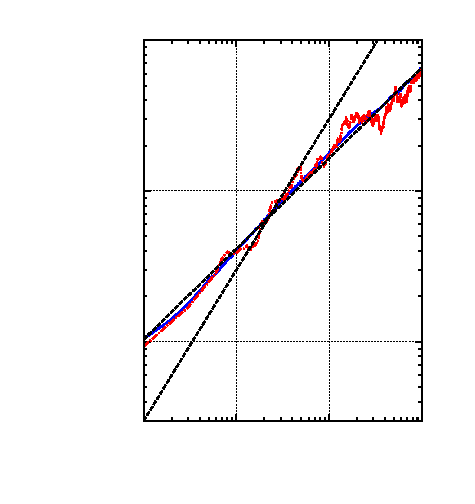
\includegraphics{MSD_beamer_ed}}%
    \gplfronttext
  \end{picture}%
\endgroup
}
\end{figure}

\end{columns}
\end{frame}

\begin{frame}
\frametitle{Frekvensanalys -- PSD}
\begin{columns}
\column{.4\textwidth}



PSD för stegen i rörelsen
\vspace{1cm}

Avvikelse från fBm


\column{.6\textwidth}
\begin{figure} %MSD dvala och logfas
\resizebox{1\textwidth}{!}{
% GNUPLOT: LaTeX picture with Postscript
\begingroup
  \makeatletter
  \providecommand\color[2][]{%
    \GenericError{(gnuplot) \space\space\space\@spaces}{%
      Package color not loaded in conjunction with
      terminal option `colourtext'%
    }{See the gnuplot documentation for explanation.%
    }{Either use 'blacktext' in gnuplot or load the package
      color.sty in LaTeX.}%
    \renewcommand\color[2][]{}%
  }%
  \providecommand\includegraphics[2][]{%
    \GenericError{(gnuplot) \space\space\space\@spaces}{%
      Package graphicx or graphics not loaded%
    }{See the gnuplot documentation for explanation.%
    }{The gnuplot epslatex terminal needs graphicx.sty or graphics.sty.}%
    \renewcommand\includegraphics[2][]{}%
  }%
  \providecommand\rotatebox[2]{#2}%
  \@ifundefined{ifGPcolor}{%
    \newif\ifGPcolor
    \GPcolortrue
  }{}%
  \@ifundefined{ifGPblacktext}{%
    \newif\ifGPblacktext
    \GPblacktexttrue
  }{}%
  % define a \g@addto@macro without @ in the name:
  \let\gplgaddtomacro\g@addto@macro
  % define empty templates for all commands taking text:
  \gdef\gplbacktext{}%
  \gdef\gplfronttext{}%
  \makeatother
  \ifGPblacktext
    % no textcolor at all
    \def\colorrgb#1{}%
    \def\colorgray#1{}%
  \else
    % gray or color?
    \ifGPcolor
      \def\colorrgb#1{\color[rgb]{#1}}%
      \def\colorgray#1{\color[gray]{#1}}%
      \expandafter\def\csname LTw\endcsname{\color{white}}%
      \expandafter\def\csname LTb\endcsname{\color{black}}%
      \expandafter\def\csname LTa\endcsname{\color{black}}%
      \expandafter\def\csname LT0\endcsname{\color[rgb]{1,0,0}}%
      \expandafter\def\csname LT1\endcsname{\color[rgb]{0,1,0}}%
      \expandafter\def\csname LT2\endcsname{\color[rgb]{0,0,1}}%
      \expandafter\def\csname LT3\endcsname{\color[rgb]{1,0,1}}%
      \expandafter\def\csname LT4\endcsname{\color[rgb]{0,1,1}}%
      \expandafter\def\csname LT5\endcsname{\color[rgb]{1,1,0}}%
      \expandafter\def\csname LT6\endcsname{\color[rgb]{0,0,0}}%
      \expandafter\def\csname LT7\endcsname{\color[rgb]{1,0.3,0}}%
      \expandafter\def\csname LT8\endcsname{\color[rgb]{0.5,0.5,0.5}}%
    \else
      % gray
      \def\colorrgb#1{\color{black}}%
      \def\colorgray#1{\color[gray]{#1}}%
      \expandafter\def\csname LTw\endcsname{\color{white}}%
      \expandafter\def\csname LTb\endcsname{\color{black}}%
      \expandafter\def\csname LTa\endcsname{\color{black}}%
      \expandafter\def\csname LT0\endcsname{\color{black}}%
      \expandafter\def\csname LT1\endcsname{\color{black}}%
      \expandafter\def\csname LT2\endcsname{\color{black}}%
      \expandafter\def\csname LT3\endcsname{\color{black}}%
      \expandafter\def\csname LT4\endcsname{\color{black}}%
      \expandafter\def\csname LT5\endcsname{\color{black}}%
      \expandafter\def\csname LT6\endcsname{\color{black}}%
      \expandafter\def\csname LT7\endcsname{\color{black}}%
      \expandafter\def\csname LT8\endcsname{\color{black}}%
    \fi
  \fi
  \setlength{\unitlength}{0.0500bp}%
  \begin{picture}(4250.00,4534.00)%
    \gplgaddtomacro\gplbacktext{%
      \csname LTb\endcsname%
      \put(1100,1750){\makebox(0,0)[r]{\strut{}\Large $10^{-3}$}}%
      \csname LTb\endcsname%
      \put(1100,3337){\makebox(0,0)[r]{\strut{}\Large $10^{-2}$}}%
      \csname LTb\endcsname%
      \put(1220,440){\makebox(0,0){\strut{}\Large 0,1}}%
      \csname LTb\endcsname%
      \put(2209,440){\makebox(0,0){\strut{}\Large 1}}%
      \csname LTb\endcsname%
      \put(3198,440){\makebox(0,0){\strut{}\Large 10}}%
      \put(160,2466){\rotatebox{-270}{\makebox(0,0){\strut{}\large PSD /[godt. enhet]}}}%
      \put(2554,140){\makebox(0,0){\strut{}\large $f$ /[Hz]}}%
    }%
    \gplgaddtomacro\gplfronttext{%
    }%
    \gplbacktext
    \put(0,0){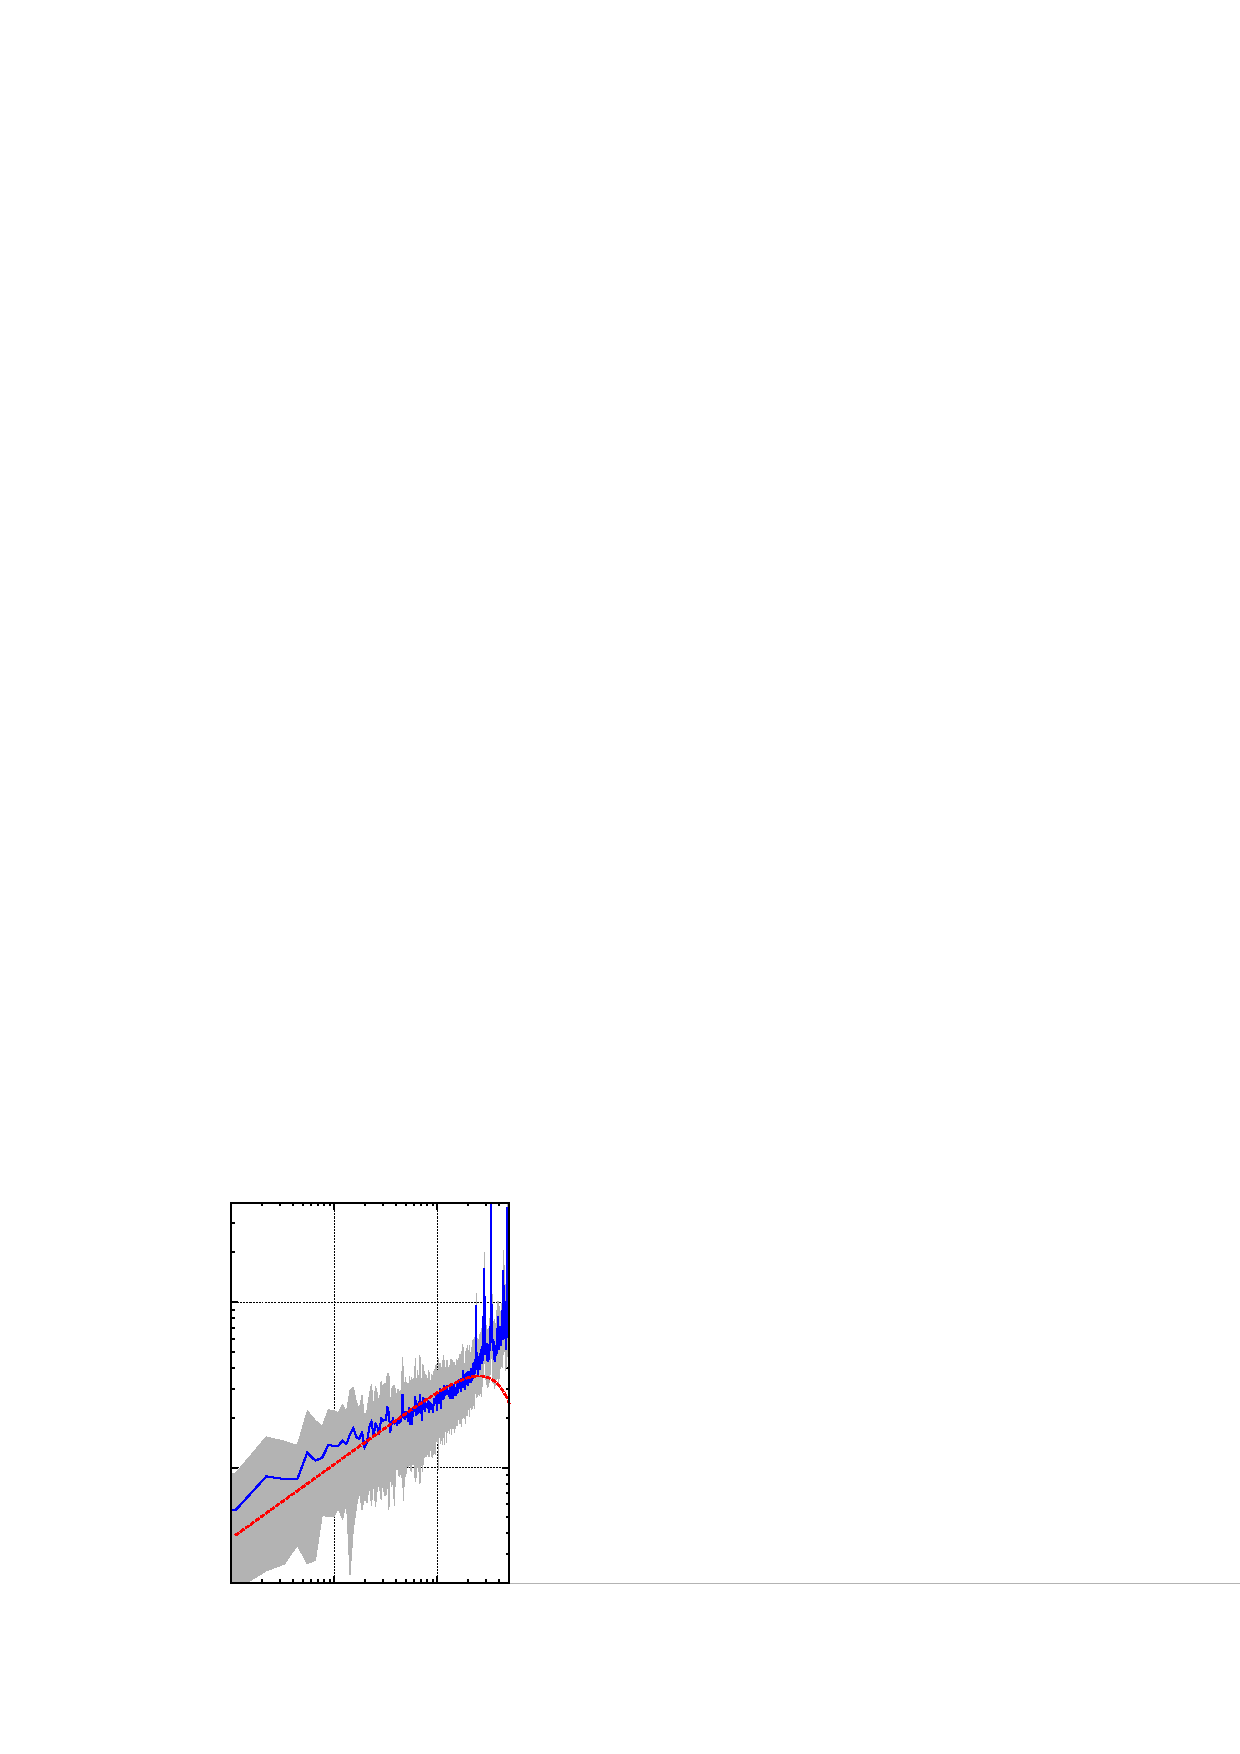
\includegraphics{PSD_beamer_ed}}%
    \gplfronttext
  \end{picture}%
\endgroup
}
\end{figure}

\end{columns}
\end{frame}


\begin{frame}
\frametitle{Skillnad mellan celler i log-fas och dvala}
\begin{columns}
\column{.4\textwidth}


Snabbare diffusion i log-fas celler
\vspace{1cm}

Cytoplasman blir mer fast i dvala?




\column{.6\textwidth}
\begin{figure} %MSD dvala och logfas
\resizebox{1\textwidth}{!}{
% GNUPLOT: LaTeX picture with Postscript
\begingroup
  \makeatletter
  \providecommand\color[2][]{%
    \GenericError{(gnuplot) \space\space\space\@spaces}{%
      Package color not loaded in conjunction with
      terminal option `colourtext'%
    }{See the gnuplot documentation for explanation.%
    }{Either use 'blacktext' in gnuplot or load the package
      color.sty in LaTeX.}%
    \renewcommand\color[2][]{}%
  }%
  \providecommand\includegraphics[2][]{%
    \GenericError{(gnuplot) \space\space\space\@spaces}{%
      Package graphicx or graphics not loaded%
    }{See the gnuplot documentation for explanation.%
    }{The gnuplot epslatex terminal needs graphicx.sty or graphics.sty.}%
    \renewcommand\includegraphics[2][]{}%
  }%
  \providecommand\rotatebox[2]{#2}%
  \@ifundefined{ifGPcolor}{%
    \newif\ifGPcolor
    \GPcolortrue
  }{}%
  \@ifundefined{ifGPblacktext}{%
    \newif\ifGPblacktext
    \GPblacktexttrue
  }{}%
  % define a \g@addto@macro without @ in the name:
  \let\gplgaddtomacro\g@addto@macro
  % define empty templates for all commands taking text:
  \gdef\gplbacktext{}%
  \gdef\gplfronttext{}%
  \makeatother
  \ifGPblacktext
    % no textcolor at all
    \def\colorrgb#1{}%
    \def\colorgray#1{}%
  \else
    % gray or color?
    \ifGPcolor
      \def\colorrgb#1{\color[rgb]{#1}}%
      \def\colorgray#1{\color[gray]{#1}}%
      \expandafter\def\csname LTw\endcsname{\color{white}}%
      \expandafter\def\csname LTb\endcsname{\color{black}}%
      \expandafter\def\csname LTa\endcsname{\color{black}}%
      \expandafter\def\csname LT0\endcsname{\color[rgb]{1,0,0}}%
      \expandafter\def\csname LT1\endcsname{\color[rgb]{0,1,0}}%
      \expandafter\def\csname LT2\endcsname{\color[rgb]{0,0,1}}%
      \expandafter\def\csname LT3\endcsname{\color[rgb]{1,0,1}}%
      \expandafter\def\csname LT4\endcsname{\color[rgb]{0,1,1}}%
      \expandafter\def\csname LT5\endcsname{\color[rgb]{1,1,0}}%
      \expandafter\def\csname LT6\endcsname{\color[rgb]{0,0,0}}%
      \expandafter\def\csname LT7\endcsname{\color[rgb]{1,0.3,0}}%
      \expandafter\def\csname LT8\endcsname{\color[rgb]{0.5,0.5,0.5}}%
    \else
      % gray
      \def\colorrgb#1{\color{black}}%
      \def\colorgray#1{\color[gray]{#1}}%
      \expandafter\def\csname LTw\endcsname{\color{white}}%
      \expandafter\def\csname LTb\endcsname{\color{black}}%
      \expandafter\def\csname LTa\endcsname{\color{black}}%
      \expandafter\def\csname LT0\endcsname{\color{black}}%
      \expandafter\def\csname LT1\endcsname{\color{black}}%
      \expandafter\def\csname LT2\endcsname{\color{black}}%
      \expandafter\def\csname LT3\endcsname{\color{black}}%
      \expandafter\def\csname LT4\endcsname{\color{black}}%
      \expandafter\def\csname LT5\endcsname{\color{black}}%
      \expandafter\def\csname LT6\endcsname{\color{black}}%
      \expandafter\def\csname LT7\endcsname{\color{black}}%
      \expandafter\def\csname LT8\endcsname{\color{black}}%
    \fi
  \fi
  \setlength{\unitlength}{0.0500bp}%
  \begin{picture}(4250.00,4534.00)%
    \gplgaddtomacro\gplbacktext{%
      \csname LTb\endcsname%
      \put(1100,1397){\makebox(0,0)[r]{\strut{}\Large $10^{-1}$}}%
      \csname LTb\endcsname%
      \put(1100,2845){\makebox(0,0)[r]{\strut{}\Large $10^{0}$}}%
      \csname LTb\endcsname%
      \put(1100,4293){\makebox(0,0)[r]{\strut{}\Large $10^{1}$}}%
      \csname LTb\endcsname%
      \put(1220,440){\makebox(0,0){\strut{}\Large 0,01}}%
      \csname LTb\endcsname%
      \put(2110,440){\makebox(0,0){\strut{}\Large 0,1}}%
      \csname LTb\endcsname%
      \put(2999,440){\makebox(0,0){\strut{}\Large 1}}%
      \csname LTb\endcsname%
      \put(3889,440){\makebox(0,0){\strut{}\Large 10}}%
      \put(160,2466){\rotatebox{-270}{\makebox(0,0){\strut{}\large MSD $/\left[\text{l.e.}^2\right]$}}}%
      \put(2554,140){\makebox(0,0){\strut{}\large $\Delta{t}$ /[s]}}%
    }%
    \gplgaddtomacro\gplfronttext{%
      \csname LTb\endcsname%
      \put(3226,1053){\makebox(0,0)[r]{\strut{}Log-fas}}%
      \csname LTb\endcsname%
      \put(3226,853){\makebox(0,0)[r]{\strut{}Dvala}}%
    }%
    \gplbacktext
    \put(0,0){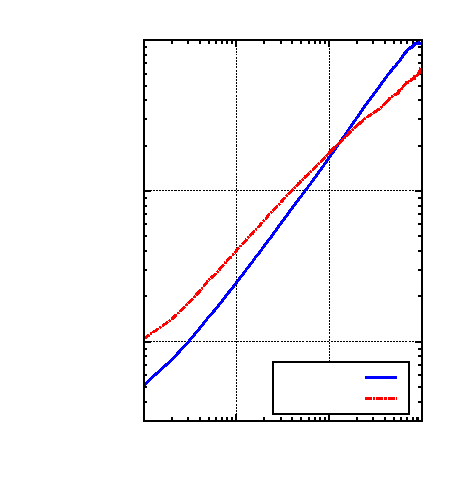
\includegraphics{MSD_beamer_skillnad}}%
    \gplfronttext
  \end{picture}%
\endgroup
}
\end{figure}

\end{columns}
\end{frame}


%%%%%%%%%%%%%%%
\section{Filamentrörelse}

\begin{frame}
\frametitle{Film av strängarna}

\end{frame}




\begin{frame}
\frametitle{WLC -- Worm-like chain}
 \begin{columns}[c]
\column{.3\textwidth} % Left column and width
%\hspace{-5mm}

 Modell för filament
\\[8mm]
 Tangentkorrelation
\\[8mm]
 Mikrokanal

\column{.7\textwidth} % Right column and width

\begin{figure}
% GNUPLOT: LaTeX picture with Postscript
\begingroup
  \makeatletter
  \providecommand\color[2][]{%
    \GenericError{(gnuplot) \space\space\space\@spaces}{%
      Package color not loaded in conjunction with
      terminal option `colourtext'%
    }{See the gnuplot documentation for explanation.%
    }{Either use 'blacktext' in gnuplot or load the package
      color.sty in LaTeX.}%
    \renewcommand\color[2][]{}%
  }%
  \providecommand\includegraphics[2][]{%
    \GenericError{(gnuplot) \space\space\space\@spaces}{%
      Package graphicx or graphics not loaded%
    }{See the gnuplot documentation for explanation.%
    }{The gnuplot epslatex terminal needs graphicx.sty or graphics.sty.}%
    \renewcommand\includegraphics[2][]{}%
  }%
  \providecommand\rotatebox[2]{#2}%
  \@ifundefined{ifGPcolor}{%
    \newif\ifGPcolor
    \GPcolortrue
  }{}%
  \@ifundefined{ifGPblacktext}{%
    \newif\ifGPblacktext
    \GPblacktexttrue
  }{}%
  % define a \g@addto@macro without @ in the name:
  \let\gplgaddtomacro\g@addto@macro
  % define empty templates for all commands taking text:
  \gdef\gplbacktext{}%
  \gdef\gplfronttext{}%
  \makeatother
  \ifGPblacktext
    % no textcolor at all
    \def\colorrgb#1{}%
    \def\colorgray#1{}%
  \else
    % gray or color?
    \ifGPcolor
      \def\colorrgb#1{\color[rgb]{#1}}%
      \def\colorgray#1{\color[gray]{#1}}%
      \expandafter\def\csname LTw\endcsname{\color{white}}%
      \expandafter\def\csname LTb\endcsname{\color{black}}%
      \expandafter\def\csname LTa\endcsname{\color{black}}%
      \expandafter\def\csname LT0\endcsname{\color[rgb]{1,0,0}}%
      \expandafter\def\csname LT1\endcsname{\color[rgb]{0,1,0}}%
      \expandafter\def\csname LT2\endcsname{\color[rgb]{0,0,1}}%
      \expandafter\def\csname LT3\endcsname{\color[rgb]{1,0,1}}%
      \expandafter\def\csname LT4\endcsname{\color[rgb]{0,1,1}}%
      \expandafter\def\csname LT5\endcsname{\color[rgb]{1,1,0}}%
      \expandafter\def\csname LT6\endcsname{\color[rgb]{0,0,0}}%
      \expandafter\def\csname LT7\endcsname{\color[rgb]{1,0.3,0}}%
      \expandafter\def\csname LT8\endcsname{\color[rgb]{0.5,0.5,0.5}}%
    \else
      % gray
      \def\colorrgb#1{\color{black}}%
      \def\colorgray#1{\color[gray]{#1}}%
      \expandafter\def\csname LTw\endcsname{\color{white}}%
      \expandafter\def\csname LTb\endcsname{\color{black}}%
      \expandafter\def\csname LTa\endcsname{\color{black}}%
      \expandafter\def\csname LT0\endcsname{\color{black}}%
      \expandafter\def\csname LT1\endcsname{\color{black}}%
      \expandafter\def\csname LT2\endcsname{\color{black}}%
      \expandafter\def\csname LT3\endcsname{\color{black}}%
      \expandafter\def\csname LT4\endcsname{\color{black}}%
      \expandafter\def\csname LT5\endcsname{\color{black}}%
      \expandafter\def\csname LT6\endcsname{\color{black}}%
      \expandafter\def\csname LT7\endcsname{\color{black}}%
      \expandafter\def\csname LT8\endcsname{\color{black}}%
    \fi
  \fi
    \setlength{\unitlength}{0.0500bp}%
    \ifx\gptboxheight\undefined%
      \newlength{\gptboxheight}%
      \newlength{\gptboxwidth}%
      \newsavebox{\gptboxtext}%
    \fi%
    \setlength{\fboxrule}{0.5pt}%
    \setlength{\fboxsep}{1pt}%
\begin{picture}(3968.00,3968.00)%
    \gplgaddtomacro\gplbacktext{%
      \csname LTb\endcsname%
      \put(740,640){\makebox(0,0)[r]{\strut{}$0,7$}}%
      \csname LTb\endcsname%
      \put(740,1669){\makebox(0,0)[r]{\strut{}$0,8$}}%
      \csname LTb\endcsname%
      \put(740,2698){\makebox(0,0)[r]{\strut{}$0,9$}}%
      \csname LTb\endcsname%
      \put(740,3727){\makebox(0,0)[r]{\strut{}$1$}}%
      \csname LTb\endcsname%
      \put(860,440){\makebox(0,0){\strut{}$0$}}%
      \csname LTb\endcsname%
      \put(1226,440){\makebox(0,0){\strut{}$2$}}%
      \csname LTb\endcsname%
      \put(1593,440){\makebox(0,0){\strut{}$4$}}%
      \csname LTb\endcsname%
      \put(1959,440){\makebox(0,0){\strut{}$6$}}%
      \csname LTb\endcsname%
      \put(2325,440){\makebox(0,0){\strut{}$8$}}%
      \csname LTb\endcsname%
      \put(2691,440){\makebox(0,0){\strut{}$10$}}%
      \csname LTb\endcsname%
      \put(3058,440){\makebox(0,0){\strut{}$12$}}%
      \csname LTb\endcsname%
      \put(3424,440){\makebox(0,0){\strut{}$14$}}%
    }%
    \gplgaddtomacro\gplfronttext{%
      \csname LTb\endcsname%
      \put(160,2183){\rotatebox{-270}{\makebox(0,0){\strut{}$\ev{\cos{\left(\theta(\Delta s)\right)}}$}}}%
      \put(2233,140){\makebox(0,0){\strut{}$\Delta s$ /[$\micro$m]}}%
    }%
    \gplbacktext
    \put(0,0){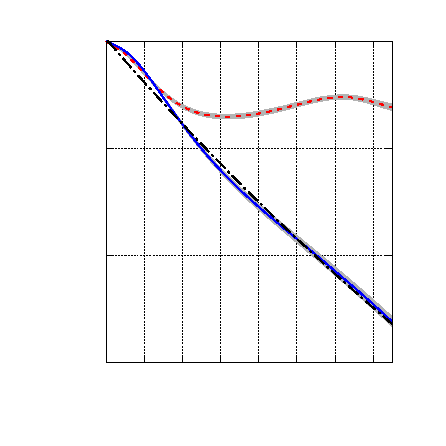
\includegraphics{tangentkorr_pres}}%
    \gplfronttext
  \end{picture}%
\endgroup

\end{figure}

\end{columns}
    
\end{frame}


\begin{frame}
\frametitle{WLC för mikrokanal}
 \begin{columns}[c]
\column{.3\textwidth} % Left column and width

Styrande differentialekvation
\vspace{8mm}

Cosinusmoder
\vspace{8mm}

Samband $\tau(k)$


\column{.7\textwidth} % Right column and width

\begin{figure}
\resizebox{!}{!}{% GNUPLOT: LaTeX picture with Postscript
\begingroup
  \makeatletter
  \providecommand\color[2][]{%
    \GenericError{(gnuplot) \space\space\space\@spaces}{%
      Package color not loaded in conjunction with
      terminal option `colourtext'%
    }{See the gnuplot documentation for explanation.%
    }{Either use 'blacktext' in gnuplot or load the package
      color.sty in LaTeX.}%
    \renewcommand\color[2][]{}%
  }%
  \providecommand\includegraphics[2][]{%
    \GenericError{(gnuplot) \space\space\space\@spaces}{%
      Package graphicx or graphics not loaded%
    }{See the gnuplot documentation for explanation.%
    }{The gnuplot epslatex terminal needs graphicx.sty or graphics.sty.}%
    \renewcommand\includegraphics[2][]{}%
  }%
  \providecommand\rotatebox[2]{#2}%
  \@ifundefined{ifGPcolor}{%
    \newif\ifGPcolor
    \GPcolortrue
  }{}%
  \@ifundefined{ifGPblacktext}{%
    \newif\ifGPblacktext
    \GPblacktexttrue
  }{}%
  % define a \g@addto@macro without @ in the name:
  \let\gplgaddtomacro\g@addto@macro
  % define empty templates for all commands taking text:
  \gdef\gplbacktext{}%
  \gdef\gplfronttext{}%
  \makeatother
  \ifGPblacktext
    % no textcolor at all
    \def\colorrgb#1{}%
    \def\colorgray#1{}%
  \else
    % gray or color?
    \ifGPcolor
      \def\colorrgb#1{\color[rgb]{#1}}%
      \def\colorgray#1{\color[gray]{#1}}%
      \expandafter\def\csname LTw\endcsname{\color{white}}%
      \expandafter\def\csname LTb\endcsname{\color{black}}%
      \expandafter\def\csname LTa\endcsname{\color{black}}%
      \expandafter\def\csname LT0\endcsname{\color[rgb]{1,0,0}}%
      \expandafter\def\csname LT1\endcsname{\color[rgb]{0,1,0}}%
      \expandafter\def\csname LT2\endcsname{\color[rgb]{0,0,1}}%
      \expandafter\def\csname LT3\endcsname{\color[rgb]{1,0,1}}%
      \expandafter\def\csname LT4\endcsname{\color[rgb]{0,1,1}}%
      \expandafter\def\csname LT5\endcsname{\color[rgb]{1,1,0}}%
      \expandafter\def\csname LT6\endcsname{\color[rgb]{0,0,0}}%
      \expandafter\def\csname LT7\endcsname{\color[rgb]{1,0.3,0}}%
      \expandafter\def\csname LT8\endcsname{\color[rgb]{0.5,0.5,0.5}}%
    \else
      % gray
      \def\colorrgb#1{\color{black}}%
      \def\colorgray#1{\color[gray]{#1}}%
      \expandafter\def\csname LTw\endcsname{\color{white}}%
      \expandafter\def\csname LTb\endcsname{\color{black}}%
      \expandafter\def\csname LTa\endcsname{\color{black}}%
      \expandafter\def\csname LT0\endcsname{\color{black}}%
      \expandafter\def\csname LT1\endcsname{\color{black}}%
      \expandafter\def\csname LT2\endcsname{\color{black}}%
      \expandafter\def\csname LT3\endcsname{\color{black}}%
      \expandafter\def\csname LT4\endcsname{\color{black}}%
      \expandafter\def\csname LT5\endcsname{\color{black}}%
      \expandafter\def\csname LT6\endcsname{\color{black}}%
      \expandafter\def\csname LT7\endcsname{\color{black}}%
      \expandafter\def\csname LT8\endcsname{\color{black}}%
    \fi
  \fi
    \setlength{\unitlength}{0.0500bp}%
    \ifx\gptboxheight\undefined%
      \newlength{\gptboxheight}%
      \newlength{\gptboxwidth}%
      \newsavebox{\gptboxtext}%
    \fi%
    \setlength{\fboxrule}{0.5pt}%
    \setlength{\fboxsep}{1pt}%
\begin{picture}(4080.00,3400.00)%
    \gplgaddtomacro\gplbacktext{%
      \csname LTb\endcsname%
      \put(560,1058){\makebox(0,0)[r]{\strut{}1}}%
      \csname LTb\endcsname%
      \put(560,2109){\makebox(0,0)[r]{\strut{}10}}%
      \csname LTb\endcsname%
      \put(560,3159){\makebox(0,0)[r]{\strut{}100}}%
      \csname LTb\endcsname%
      \put(680,440){\makebox(0,0){\strut{}0}}%
      \csname LTb\endcsname%
      \put(1187,440){\makebox(0,0){\strut{}0.2}}%
      \csname LTb\endcsname%
      \put(1693,440){\makebox(0,0){\strut{}0.4}}%
      \csname LTb\endcsname%
      \put(2200,440){\makebox(0,0){\strut{}0.6}}%
      \csname LTb\endcsname%
      \put(2706,440){\makebox(0,0){\strut{}0.8}}%
      \csname LTb\endcsname%
      \put(3213,440){\makebox(0,0){\strut{}1}}%
      \csname LTb\endcsname%
      \put(3719,440){\makebox(0,0){\strut{}1.2}}%
    }%
    \gplgaddtomacro\gplfronttext{%
      \csname LTb\endcsname%
      \put(160,1899){\rotatebox{-270}{\makebox(0,0){\strut{}$\tau$ /[s]}}}%
      \put(2199,140){\makebox(0,0){\strut{}$k$ /[$\micro$m$^{-1}$]}}%
    }%
    \gplbacktext
    \put(0,0){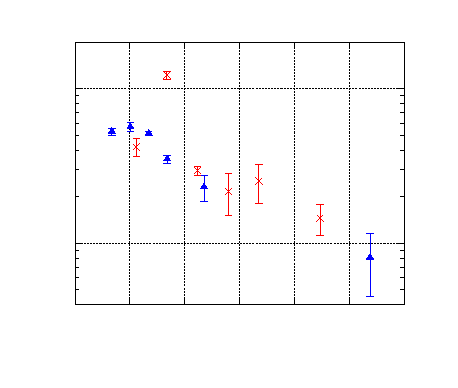
\includegraphics{cosktauconf_pres}}%
    \gplfronttext
  \end{picture}%
\endgroup
}
% \caption{}
\end{figure}

%\begin{figure}
%\resizebox{!}{3cm}{% GNUPLOT: LaTeX picture with Postscript
\begingroup
  \makeatletter
  \providecommand\color[2][]{%
    \GenericError{(gnuplot) \space\space\space\@spaces}{%
      Package color not loaded in conjunction with
      terminal option `colourtext'%
    }{See the gnuplot documentation for explanation.%
    }{Either use 'blacktext' in gnuplot or load the package
      color.sty in LaTeX.}%
    \renewcommand\color[2][]{}%
  }%
  \providecommand\includegraphics[2][]{%
    \GenericError{(gnuplot) \space\space\space\@spaces}{%
      Package graphicx or graphics not loaded%
    }{See the gnuplot documentation for explanation.%
    }{The gnuplot epslatex terminal needs graphicx.sty or graphics.sty.}%
    \renewcommand\includegraphics[2][]{}%
  }%
  \providecommand\rotatebox[2]{#2}%
  \@ifundefined{ifGPcolor}{%
    \newif\ifGPcolor
    \GPcolortrue
  }{}%
  \@ifundefined{ifGPblacktext}{%
    \newif\ifGPblacktext
    \GPblacktexttrue
  }{}%
  % define a \g@addto@macro without @ in the name:
  \let\gplgaddtomacro\g@addto@macro
  % define empty templates for all commands taking text:
  \gdef\gplbacktext{}%
  \gdef\gplfronttext{}%
  \makeatother
  \ifGPblacktext
    % no textcolor at all
    \def\colorrgb#1{}%
    \def\colorgray#1{}%
  \else
    % gray or color?
    \ifGPcolor
      \def\colorrgb#1{\color[rgb]{#1}}%
      \def\colorgray#1{\color[gray]{#1}}%
      \expandafter\def\csname LTw\endcsname{\color{white}}%
      \expandafter\def\csname LTb\endcsname{\color{black}}%
      \expandafter\def\csname LTa\endcsname{\color{black}}%
      \expandafter\def\csname LT0\endcsname{\color[rgb]{1,0,0}}%
      \expandafter\def\csname LT1\endcsname{\color[rgb]{0,1,0}}%
      \expandafter\def\csname LT2\endcsname{\color[rgb]{0,0,1}}%
      \expandafter\def\csname LT3\endcsname{\color[rgb]{1,0,1}}%
      \expandafter\def\csname LT4\endcsname{\color[rgb]{0,1,1}}%
      \expandafter\def\csname LT5\endcsname{\color[rgb]{1,1,0}}%
      \expandafter\def\csname LT6\endcsname{\color[rgb]{0,0,0}}%
      \expandafter\def\csname LT7\endcsname{\color[rgb]{1,0.3,0}}%
      \expandafter\def\csname LT8\endcsname{\color[rgb]{0.5,0.5,0.5}}%
    \else
      % gray
      \def\colorrgb#1{\color{black}}%
      \def\colorgray#1{\color[gray]{#1}}%
      \expandafter\def\csname LTw\endcsname{\color{white}}%
      \expandafter\def\csname LTb\endcsname{\color{black}}%
      \expandafter\def\csname LTa\endcsname{\color{black}}%
      \expandafter\def\csname LT0\endcsname{\color{black}}%
      \expandafter\def\csname LT1\endcsname{\color{black}}%
      \expandafter\def\csname LT2\endcsname{\color{black}}%
      \expandafter\def\csname LT3\endcsname{\color{black}}%
      \expandafter\def\csname LT4\endcsname{\color{black}}%
      \expandafter\def\csname LT5\endcsname{\color{black}}%
      \expandafter\def\csname LT6\endcsname{\color{black}}%
      \expandafter\def\csname LT7\endcsname{\color{black}}%
      \expandafter\def\csname LT8\endcsname{\color{black}}%
    \fi
  \fi
    \setlength{\unitlength}{0.0500bp}%
    \ifx\gptboxheight\undefined%
      \newlength{\gptboxheight}%
      \newlength{\gptboxwidth}%
      \newsavebox{\gptboxtext}%
    \fi%
    \setlength{\fboxrule}{0.5pt}%
    \setlength{\fboxsep}{1pt}%
\begin{picture}(4080.00,3400.00)%
    \gplgaddtomacro\gplbacktext{%
      \csname LTb\endcsname%
      \put(560,1058){\makebox(0,0)[r]{\strut{}1}}%
      \csname LTb\endcsname%
      \put(560,2109){\makebox(0,0)[r]{\strut{}10}}%
      \csname LTb\endcsname%
      \put(560,3159){\makebox(0,0)[r]{\strut{}100}}%
      \csname LTb\endcsname%
      \put(680,440){\makebox(0,0){\strut{}0}}%
      \csname LTb\endcsname%
      \put(1187,440){\makebox(0,0){\strut{}0.2}}%
      \csname LTb\endcsname%
      \put(1693,440){\makebox(0,0){\strut{}0.4}}%
      \csname LTb\endcsname%
      \put(2200,440){\makebox(0,0){\strut{}0.6}}%
      \csname LTb\endcsname%
      \put(2706,440){\makebox(0,0){\strut{}0.8}}%
      \csname LTb\endcsname%
      \put(3213,440){\makebox(0,0){\strut{}1}}%
      \csname LTb\endcsname%
      \put(3719,440){\makebox(0,0){\strut{}1.2}}%
    }%
    \gplgaddtomacro\gplfronttext{%
      \csname LTb\endcsname%
      \put(160,1899){\rotatebox{-270}{\makebox(0,0){\strut{}$\tau$ /[s]}}}%
      \put(2199,140){\makebox(0,0){\strut{}$k$ /[$\micro$m$^{-1}$]}}%
    }%
    \gplbacktext
    \put(0,0){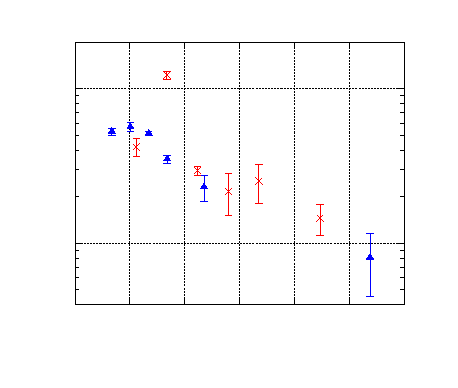
\includegraphics{cosktauconf_pres}}%
    \gplfronttext
  \end{picture}%
\endgroup
}
% \caption{}
%\end{figure}

\end{columns}

\end{frame}


\begin{frame}
\frametitle{Kovariansmatrisen -- Egenmoder}

\begin{columns}[c]
\column{.4\textwidth} % Left column and width
Kovariansmatris
\begin{itemize}[label={$\bullet$}]
    \item Statistisk information
    \item Egenvektorer
\end{itemize}
\vspace{1cm}

$\cos (ks)$ $\impl$ Egenvektor
\column{.7\textwidth} % Right column and width

\begin{figure}
% GNUPLOT: LaTeX picture with Postscript
\begingroup
  \makeatletter
  \providecommand\color[2][]{%
    \GenericError{(gnuplot) \space\space\space\@spaces}{%
      Package color not loaded in conjunction with
      terminal option `colourtext'%
    }{See the gnuplot documentation for explanation.%
    }{Either use 'blacktext' in gnuplot or load the package
      color.sty in LaTeX.}%
    \renewcommand\color[2][]{}%
  }%
  \providecommand\includegraphics[2][]{%
    \GenericError{(gnuplot) \space\space\space\@spaces}{%
      Package graphicx or graphics not loaded%
    }{See the gnuplot documentation for explanation.%
    }{The gnuplot epslatex terminal needs graphicx.sty or graphics.sty.}%
    \renewcommand\includegraphics[2][]{}%
  }%
  \providecommand\rotatebox[2]{#2}%
  \@ifundefined{ifGPcolor}{%
    \newif\ifGPcolor
    \GPcolortrue
  }{}%
  \@ifundefined{ifGPblacktext}{%
    \newif\ifGPblacktext
    \GPblacktexttrue
  }{}%
  % define a \g@addto@macro without @ in the name:
  \let\gplgaddtomacro\g@addto@macro
  % define empty templates for all commands taking text:
  \gdef\gplbacktext{}%
  \gdef\gplfronttext{}%
  \makeatother
  \ifGPblacktext
    % no textcolor at all
    \def\colorrgb#1{}%
    \def\colorgray#1{}%
  \else
    % gray or color?
    \ifGPcolor
      \def\colorrgb#1{\color[rgb]{#1}}%
      \def\colorgray#1{\color[gray]{#1}}%
      \expandafter\def\csname LTw\endcsname{\color{white}}%
      \expandafter\def\csname LTb\endcsname{\color{black}}%
      \expandafter\def\csname LTa\endcsname{\color{black}}%
      \expandafter\def\csname LT0\endcsname{\color[rgb]{1,0,0}}%
      \expandafter\def\csname LT1\endcsname{\color[rgb]{0,1,0}}%
      \expandafter\def\csname LT2\endcsname{\color[rgb]{0,0,1}}%
      \expandafter\def\csname LT3\endcsname{\color[rgb]{1,0,1}}%
      \expandafter\def\csname LT4\endcsname{\color[rgb]{0,1,1}}%
      \expandafter\def\csname LT5\endcsname{\color[rgb]{1,1,0}}%
      \expandafter\def\csname LT6\endcsname{\color[rgb]{0,0,0}}%
      \expandafter\def\csname LT7\endcsname{\color[rgb]{1,0.3,0}}%
      \expandafter\def\csname LT8\endcsname{\color[rgb]{0.5,0.5,0.5}}%
    \else
      % gray
      \def\colorrgb#1{\color{black}}%
      \def\colorgray#1{\color[gray]{#1}}%
      \expandafter\def\csname LTw\endcsname{\color{white}}%
      \expandafter\def\csname LTb\endcsname{\color{black}}%
      \expandafter\def\csname LTa\endcsname{\color{black}}%
      \expandafter\def\csname LT0\endcsname{\color{black}}%
      \expandafter\def\csname LT1\endcsname{\color{black}}%
      \expandafter\def\csname LT2\endcsname{\color{black}}%
      \expandafter\def\csname LT3\endcsname{\color{black}}%
      \expandafter\def\csname LT4\endcsname{\color{black}}%
      \expandafter\def\csname LT5\endcsname{\color{black}}%
      \expandafter\def\csname LT6\endcsname{\color{black}}%
      \expandafter\def\csname LT7\endcsname{\color{black}}%
      \expandafter\def\csname LT8\endcsname{\color{black}}%
    \fi
  \fi
    \setlength{\unitlength}{0.0500bp}%
    \ifx\gptboxheight\undefined%
      \newlength{\gptboxheight}%
      \newlength{\gptboxwidth}%
      \newsavebox{\gptboxtext}%
    \fi%
    \setlength{\fboxrule}{0.5pt}%
    \setlength{\fboxsep}{1pt}%
\begin{picture}(4534.00,3968.00)%
    \gplgaddtomacro\gplbacktext{%
      \csname LTb\endcsname%
      \put(660,924){\makebox(0,0)[r]{\strut{}$-0,1$}}%
      \csname LTb\endcsname%
      \put(660,1728){\makebox(0,0)[r]{\strut{}$0$}}%
      \csname LTb\endcsname%
      \put(660,2532){\makebox(0,0)[r]{\strut{}$0,1$}}%
      \csname LTb\endcsname%
      \put(660,3336){\makebox(0,0)[r]{\strut{}$0,2$}}%
      \csname LTb\endcsname%
      \put(780,440){\makebox(0,0){\strut{}$0$}}%
      \csname LTb\endcsname%
      \put(1265,440){\makebox(0,0){\strut{}$5$}}%
      \csname LTb\endcsname%
      \put(1749,440){\makebox(0,0){\strut{}$10$}}%
      \csname LTb\endcsname%
      \put(2234,440){\makebox(0,0){\strut{}$15$}}%
      \csname LTb\endcsname%
      \put(2719,440){\makebox(0,0){\strut{}$20$}}%
      \csname LTb\endcsname%
      \put(3204,440){\makebox(0,0){\strut{}$25$}}%
      \csname LTb\endcsname%
      \put(3688,440){\makebox(0,0){\strut{}$30$}}%
      \csname LTb\endcsname%
      \put(4173,440){\makebox(0,0){\strut{}$35$}}%
    }%
    \gplgaddtomacro\gplfronttext{%
      \csname LTb\endcsname%
      \put(200,2183){\rotatebox{-270}{\makebox(0,0){\strut{}$B_i(s)$}}}%
      \put(2476,140){\makebox(0,0){\strut{}$s$ /[$\micro$m]}}%
    }%
    \gplbacktext
    \put(0,0){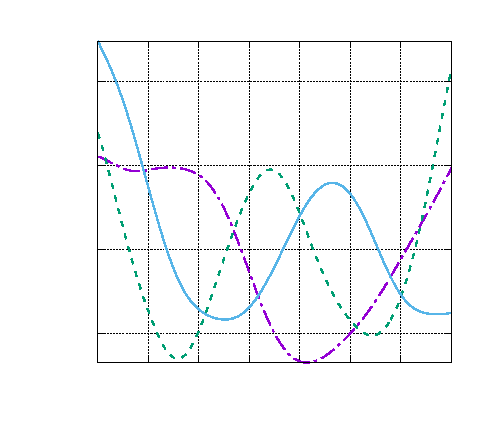
\includegraphics{moder_pres}}%
    \gplfronttext
  \end{picture}%
\endgroup

 %\caption{}
\end{figure}

\end{columns}
    
\end{frame}

\section{Sammanfattning}
\begin{frame}
\frametitle{Sammanfattning}

\begin{itemize}[label={$\bullet$}]
    
 \item{Det saknas en fullständig modell för partikelrörelse}
\\[8mm]
 \item{Diffusion sker långsammare i celler i dvala}
\\[8mm]
 \item{Strängrörelsen representeras väl av egenmoderna}
\\[8mm]
\item{Egenmoderna liknar de teoretiska cosinusmoderna}

\end{itemize}


\end{frame}

\begin{frame}
\frametitle{Till sist...}
    \begin{center}
    \huge Tack! 
    \end{center}
\end{frame}


\end{document}




